\section{Planen als logische Inferenz}

\paragraph{Klassisches KI-PLanen: Blocks World}

``Blocks World'' ist ein klassisches Beispiel, wenn es um Planung mit KI geht. In der Welt der Bl�cke gibt es einige identifizierbare Bl�cke, A, B, C, \dots, die nebeneinander liegen oder �bereinander gestapelt sind. Es gibt auch einen Greifer, der einen Block aufnehmen kann, solange kein anderer Block auf dem zu aufnehmenden Block gestapelt ist.

\begin{figure}[H]
    \centering
    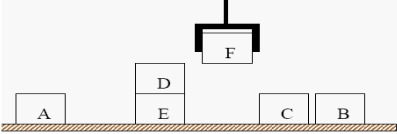
\includegraphics[width=0.7\textwidth]{figures/kap9/blocks-world.png}
    \caption{Darstellung von Blocks World}
    \label{fig:blocks-world}
\end{figure}

Da die Startpositionen und die Zielkonfiguration der Bl�cke im Stil der Pr�dikatenlogik 1. Stufe (siehe Kapitel~\ref{section:pl1}) als Konjunktion von Eigenschaften gegeben sind, wird eine Folge von Aktionen f�r den Greifer gesucht, die die Konfigurations�nderung von der Startposition zur Zielposition bewirken kann.

\paragraph{L�sen mittels logische Inferenz}

Eine M�glichkeit, eine L�sung f�r dieses Problem zu finden, ist das Planen als logische Inferenz. Die klassische Pr�dikatenlogik ist f�r dynamische Prozesse wie diesen nicht geeignet. Um dies zu umgehen, k�nnen Zust�nde, \(s\), als Objekte mit bestimmten Eigenschaften \(P(s)\) und \(Q(s)\) betrachtet werden. Aktion, A kann als eine �bergangsrelation \(A(s_i, s_k)\) gebildet werden, die den Zustand \(s_i\) auf \(s_k\) abbildet. Die Aktionen k�nnen dann als Regeln in der Form:

\[(P(s_i) \wedge A(s_i, s_k)) => Q(s_k)\]

Diese Art der Planung hat viele Vorteile: Die Formulierung des Problems kann sich in diesem Fall auf die Formulierung von Aktionen und den Ziel- und Startzustand beschr�nken und ein allgemeiner Theorembeweiser kann verwendet werden, um das Problem zu l�sen, indem das durch die Inferenzschritte erzeugte Protokoll zur�ckverfolgt wird.

Dieser Ansatz hat jedoch auch einige Nachteile. N�mlich die Tatsache, dass man eine Reihe von Problemen bew�ltigen muss, die mit der Verwendung eines Planoperators einhergehen. Diese Reihe von Problemen besteht im Wesentlichen darin, dass es nicht m�glich ist, die Auswirkungen einer Handlung zu beschreiben, insbesondere in der realen Welt, wenn einige Handlungen fehlschlagen. Au�erdem ist die Planerstellung nicht besonders effizient, da sie einen allgemeinen L�ser verwendet.